% TODO:
% 1. fix the conclusion section about the network results

\documentclass[12pt]{article}

% Language setting
% Replace `english' with e.g. `spanish' to change the document language
\usepackage[english]{babel}

% Set page size and margins
% Replace `letterpaper' with`a4paper' for UK/EU standard size
\usepackage[letterpaper,top=2cm,bottom=2cm,left=3cm,right=3cm,marginparwidth=1.75cm]{geometry}

% Useful packages
\usepackage{amsmath}
\usepackage{graphicx}
\usepackage[colorlinks=true, allcolors=blue]{hyperref}

\usepackage{xcolor}
\definecolor{light-gray}{gray}{0.95}
\newcommand{\code}[1]{\colorbox{light-gray}{\texttt{#1}}}


\title{Quantifying CPU and Network savings in Computational Storage Systems}
\author{Jayjeet Chakraborty}

\begin{document}
\maketitle

\begin{abstract}
Computational Storage allows offloading compute operations from clients to servers to be able to mitigate performance implications due to client-side CPU bottleneck and hampered scalability. Since the compute capability of the client is distributed across the storage tier in computational storage, we might be able to use cheap low power CPUs on the storage servers, to be able to retrieve equivalent performance as client side computation while enjoying benefits of compute offloading such as reduced network bandwidth. In this paper, we aim to find out how much resource savings in terms of CPU and Network can one achieve by adopting computational storage. 
\end{abstract}

\section{Introduction}

In the past decade, I/O hardware like the Disks and the Network interconnects have become faster than ever. With the introduction of protocols such as NVMe, SSDs can now sustain a throughput of $2$-$3$ GB/s. Also, with innovations in networking hardware and RDMA technologies like Infiniband and RoCE becoming mainstream, it is common to find link speeds of $25$-$100$ Gbps in modern data centers. But, with Moore's law coming to an end, CPU processing capabilities have failed to keep up with the fast I/O devices, causing the performance bottleneck to shift from the I/O devices to the CPU. The notion of "a fast CPU and slow disk" is rendered invalid in today's high-performance systems as shown by Trivedi et. al. One solution to this problem is to move the processing from the client to the storage layer, so that the single client CPU is no more the bottleneck. Offloading compute to the storage layer gets the computation access to the storage layer CPUs in a scalable manner enabling the system to benefit from the high-performance I/O devices. Another benefit of using computational storage is that it reduces unnecessary data movement from the storage to the client resulting in network bandwidth savings, reduced latency, and high throughput. Since, the computation is taken from the client and distributed amongst the storage layer, every storage server does a fraction of the total work and does not utilize all of its CPU cycles. Also, when only the result of a computation is sent back to the client from the storage layer, only a fraction of the network bandwidth is used. In this paper, we aim to quantify the resource savings in terms of CPU and network bandwidth that one can expect to get by using computational storage. We aim to find out if adopting computational storage can help lower infrastructure costs by enabling the use of cheaper CPUs and interconnects while preserving competitive performance. We use Skyhook~\cite{chakraborty2022skyhook}, as our candidate computational storage system for performing this study. It is described in detail in Section~\ref{sec:background}. Overall, the paper is organized as follows: Section~\ref{sec:background} goes over the background information that is required to understand this paper, Section~\ref{sec:experiments} describes the experiments in detail along with the observations, and finally Section~\ref{sec:future-and-concl} discusses future work and concluding thoughts.

\section{Background}
\label{sec:background}
This section discusses in detail the different systems and technologies that we use to perform our experiments.

\subsection{Apache Arrow}
\textit{Apache Arrow} is an in-memory columnar format optimized for efficient analytics operations on modern hardware. It describes a standard data format for exchanging structured data between different systems without serialization or deserialization. The Arrow format allows compute engines and query execution engines to maximize their efficiency when scanning and iterating large chunks of data. The contiguous columnar layout of Arrow enables vectorization using the latest SIMD operations on modern hardware. Besides being an in-memory format, it is also a collection of different data processing components that allow building parts of a data processing system. Some of the most-used components are Flight, a gRPC-based data transfer protocol~\cite{flight}; Feather, A Arrow-based columnar persistent storage format~\cite{feather}; Gandiva, An LLVM-based expression compiler~\cite{gandiva}; Dataset API, An abstraction for realizing datasets over a directory of files~\cite{ArrowDatasetDocs}. Arrow is also language-independent as it has APIs in several different programming languages such as C++, Java, Python, Rust, R, JavaScript, and Julia. Several popular data processing systems such as Spark, Dask~\cite{Dask}, Ray~\cite{Ray}, Pandas, Parquet~\cite{parquet} have added support for Arrow data and Arrow data sources~\cite{jc2022skyhook}.

\subsection{Ceph}
\begin{figure}[h]
\centering
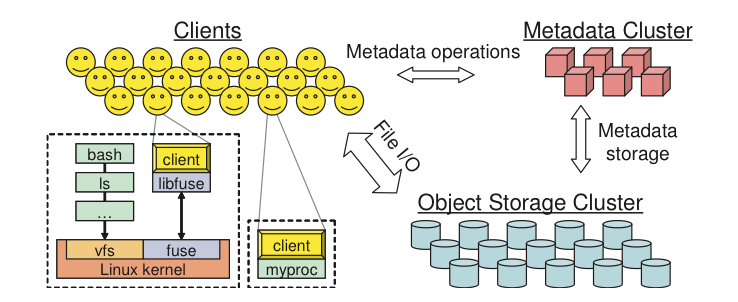
\includegraphics[width=\textwidth]{figs/cepharch.png}
\caption{Architecture of Ceph ~\cite{weil2006ceph}.}
\label{fig:ceph-arch}
\end{figure}

\textit{Ceph} is a petabyte-scale distributed and programmable object storage system providing $3$-in-$1$ interfaces for object, file, and block-level storage. Ceph was developed as a part of a Ph.D. thesis at UC Santa Cruz and was first published in 2006. Ceph does not use any other filesystems internally; rather, it manages the HDDs and SSDs directly with its custom storage backend, BlueStore, part of its RADOS~\cite{weil2007rados} object store. Ceph was developed for commodity hardware, and hence it can replicate data across a cluster, employing several techniques such as erasure coding, replication, and snapshots. Ceph is unique as it does not have a single point of failure. This is because of the CRUSH~\cite{weil2006crush} map feature that Ceph provides. CRUSH maps contain object-OSD mappings, which the Ceph client uses to calculate the location of an object in a Ceph cluster. After figuring out the location of an object, the client directly connects to a Ceph OSD and reads the object. Ceph also provides a plugin-based object store extension mechanism through its Object Class SDK~\cite{objectclasssdk}. This SDK allows writing embeddable plugins (in the form of shared libraries) in C++ and Lua containing logic to access and modify objects inside the storage servers within the RADOS I/O path. The SDK provides a subset of POSIX-like system calls such as ~\code{cls\_cxx\_read}, ~\code{cls\_cxx\_write}, and ~\code{cls\_cxx\_stat} to be able to read, write, and stat objects respectively. This SDK is heavily used by several Ceph components such as Ceph RBD (Rados Block Device) and CephFS (the Ceph filesystem). The architecture of Ceph is given in Figure~\ref{fig:ceph-arch}.

\subsection{Skyhook}
\begin{figure}[h]
\centering
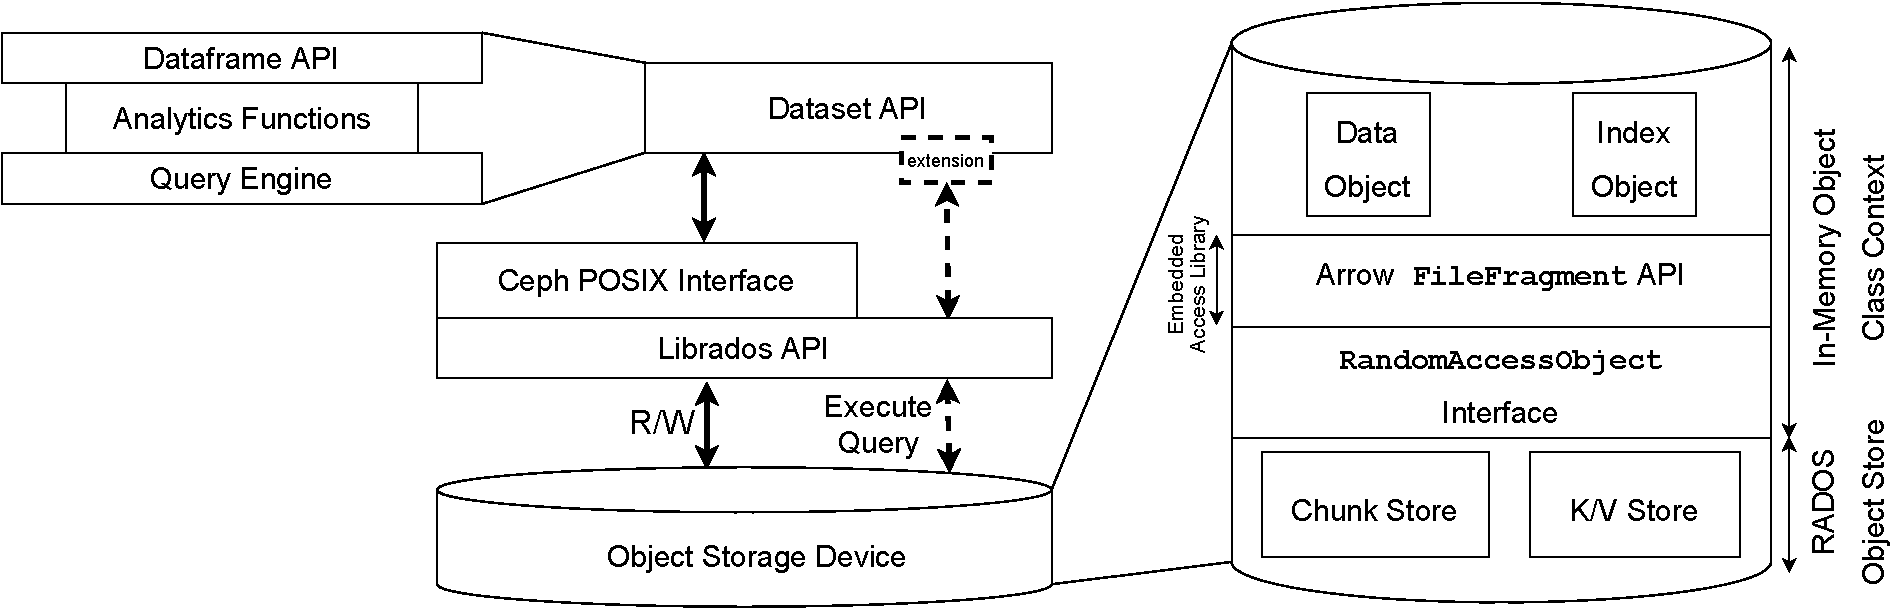
\includegraphics[width=\textwidth]{figs/implarch.pdf}
\caption{Architecture of Skyhook ~\cite{jc2022skyhook}.}
\label{fig:skyhook-arch}
\end{figure}

\textit{Skyhook} is a programmable storage system built on top of Ceph that can offload query executions from the client to the storage layer. Skyhook supports scanning datasets containing files of different formats such as Parquet, Feather, CSV, JSON, or any other format as long as they are supported by Apache Arrow. Skyhook is built as a storage-side plugin for Ceph, which, when embedded inside Ceph OSDs in the form of shared libraries, allows executing queries within the Ceph storage servers. Skyhook is exposed to the clients using a Arrow ~\code{FileFormat} API extension called the \code{SkyhookFileFormat} API. This API, when used with the Arrow ~\code{Dataset} API, allows offloading dataset scans instantly. Internally, ~\code{SkyhookFileFormat} leverages Ceph filesystem metadata containing file striping information to map files in CephFS to RADOS objects and applies computation on those objects directly, bypassing the POSIX layer. In the storage plugin, we reuse the ~\code{ParquetFileFormat} of Arrow out-of-the-box to scan RADOS objects containing Parquet binary data. Generally, Arrow APIs cannot scan RADOS objects. However, we make this possible by creating a thin random-access filesystem shim called the ~\code{RandomAccessObject} API that wraps a RADOS object, keeps track of the file pointer, and provides a file-like view over the objects. This interface plugs into Arrow APIs seamlessly and allows scanning objects as files. One exception for Skyhook is that it requires files to be written in a specific way. To be able to scan Parquet files with Skyhook, they should be self-contained within a single RADOS object. This $1:1$ mapping is required to be able to translate filenames into object IDs easily and to let Arrow APIs scan a RADOS object as a complete Parquet file, as Arrow APIs cannot scan multiple physical files as a single logical file. To ensure every file goes into a single object while writing files to CephFS, we change the stripe unit of CephFS to match the size of the Parquet files being written. The architecture of Skyhook is given in Figure~\ref{fig:skyhook-arch}.

\section{Experiments}
\label{sec:experiments}
In this section, we describe our experiment setup, how we perform our experiments, and our observations. We perform $2$ kinds of experiments to show CPU and network bandwidth savings from offloading compute to the storage layer. The experiments were performed on CloudLab, the NSF-funded bare-metal-as-a-service infrastructure. For our
experiments, we exclusively used machines with an 8-core
Intel Xeon D-1548 2.0 GHz processor (with hyperthreading
enabled), 64 GB DRAM, a 256 GB NVMe drive, and a 10 GbE
network interface. These bare-metal servers are codenamed
“m510” in CloudLab. We used Ceph octopus v15.2.16 on Ubuntu 20.04 (Linux kernel 5.4.0-100-generic) along with Skyhook v0.4.0 for our experiments. We used Ceph clusters of size 1, 8, 16 for our experiments as these sizes are pretty common for a standard Ceph deployment. Every storage server had a single Ceph OSD running on the local NVMe drive. We configured the OSDs to use 8 threads to prevent any contention due to hyperthreading in the storage servers. The number of placement groups was increased from 128 to 512 to prevent contention from PG locking. A CephFS interface was created on a replicated data pool and was mounted in user mode using the ~\code{ceph-fuse} utility. We repeat each experiment $5$-$10$ times to produce somewhat statistically significant results. 
\subsection{CPU Frequency}

\begin{figure}[htp]

\centering
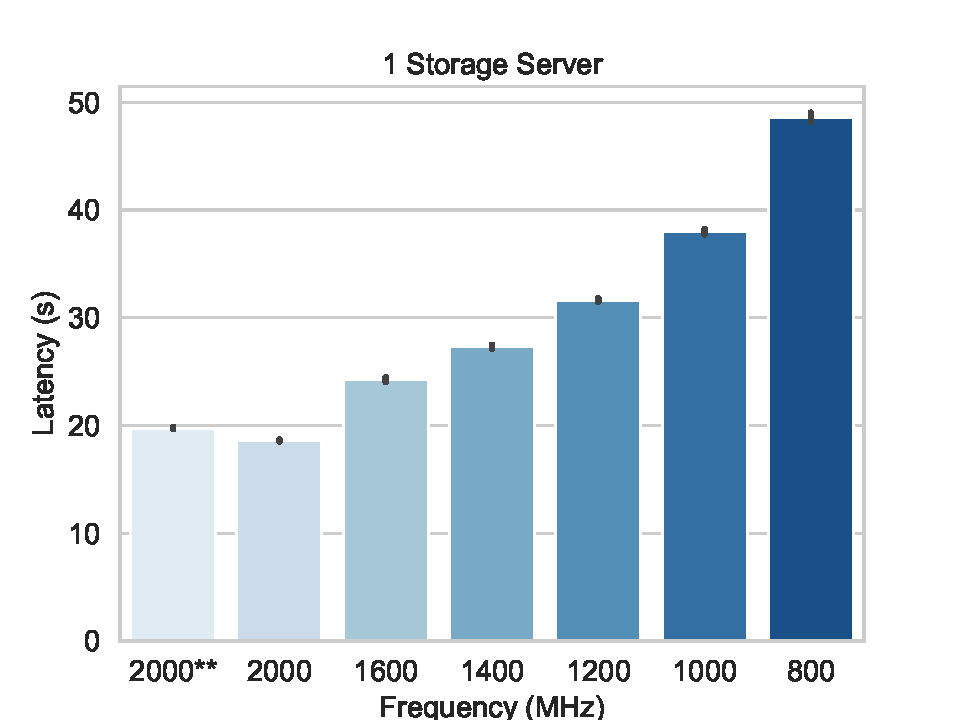
\includegraphics[width=.63\textwidth]{figs/plot_1.pdf}\hfill
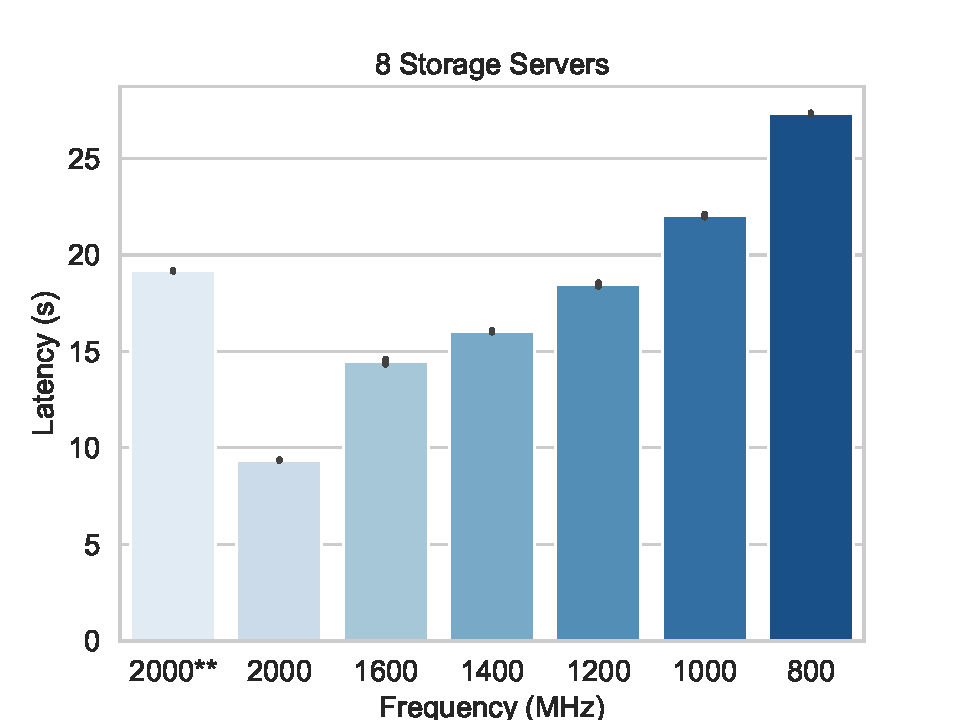
\includegraphics[width=.63\textwidth]{figs/plot_8.pdf}\hfill
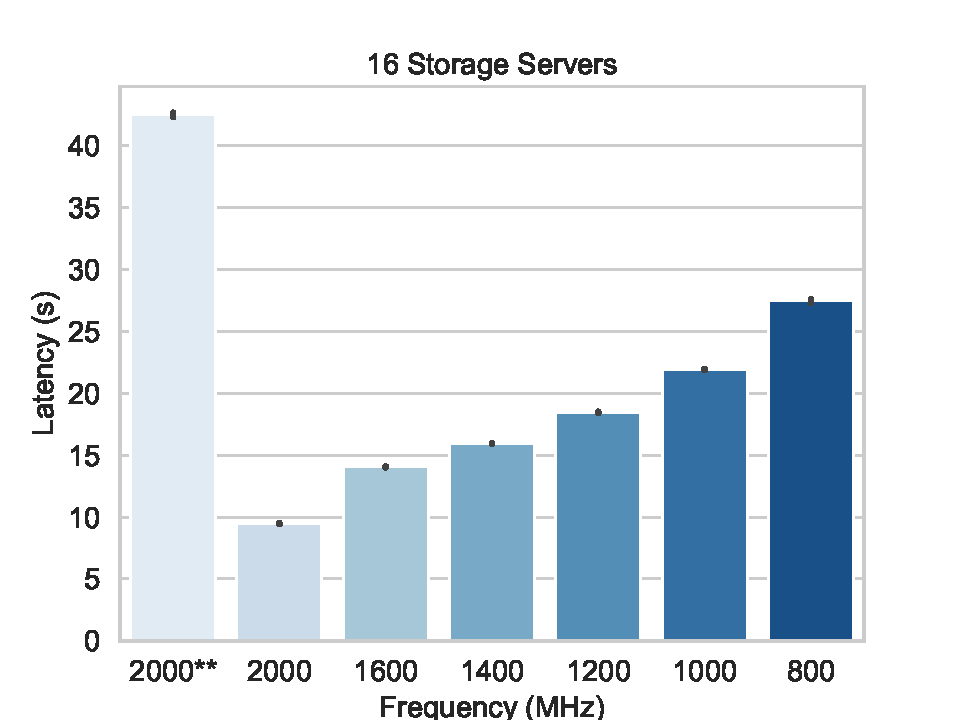
\includegraphics[width=.63\textwidth]{figs/plot_16.pdf}

\caption{Latency vs Storage server CPU frequency plot for a Skyhook (storage-side) query execution with $1$\% query selectivity. One exception is that, the leftmost bar (**) in every plot shows the latency of a client-side execution with a $2000$ MHz CPU serving as the baseline.}
\label{fig:cpu}

\end{figure}

One of the goals of this paper is to find out the minimum amount of processing capability required per storage server CPU to be able to generate the same performance as a fast client side CPU can provide. We take Skyhook as our computational storage system and execute queries to select $1$\% of the rows both on the client and the server side. We use the ~\code{cpufrequtils} toolchain provided by Linux to change the CPU speed on the storage servers. We discuss how to use this tool in detail in Appendix~\ref{sec:app-cpu}. Since the lowest frequency that we can set our cores at was $800$ MHz, we performed our experiments in the frequency range of $800$ MHz and $2000$ MHz. We repeated this experiment on a Skyhook cluster of $1$, $8$, and $16$ storage servers respectively to find out how much CPU one can save per server by scaling out. We performed weak scaling by increasing our dataset size slowly from $460$ to $920$ files as we scaled out from $8$ to $16$ storage servers. Our dataset was comprised of replicated $64$MB uncompressed Parquet files containing data from the infamous NYC taxi dataset. Each file consisted of $2.6$ million rows and $17$ columns. For every cluster size, we start with a client side query execution with both the client and server side CPUs at $2000$ MHz. Then we perform a storage side query execution with both the sides still at $2000$ MHz. After that we slowly tune down the storage side CPU frequencies by a difference of $200$ MHz at each step and perform storage side query executions for each step. We repeat this till we find the query performance to match the client side query execution at $2000$ MHz on both sides. We observe that in a single server Skyhook cluster, we cannot use a low power CPU on the storage because there is only a single storage layer CPU to match the client CPU, so both their frequencies should be the same. On the other hand, when we have a cluster with $8$ and $16$ servers respectively, we can tune down the CPU frequencies to $1200$ MHz and $800$ MHz respectively and still get similar or better performance. Ideally, for the $16$ server cases, we should have been fine running the storage server CPUs at $600$ MHz but the kernel only allowed us to tune down the CPUs till $800$ MHz. Figure~\ref{fig:cpu} shows our observations for this experiment.

\subsection{Network Bandwidth}



\subsection{Cost}

\section{Conclusion and Future Work}
\label{sec:future-and-concl}
This paper studies resource savings that computational storage systems can bring in terms of CPU and Network bandwidth as compared to systems where computation happen on the client. We use Skyhook as our candidate computation storage system for performing the experiments. Our results show that using computational storage certainly helps save CPU resources on the storage servers and the savings increases as we scale out and distribute our computation across more storage servers. This shows that there is a real possibility of using low-power chips such as FPGAs embedded on SSDs for compute offloading. We also show that moving to computational storage allows saving network bandwidth, which becomes particularly important in data centers where the storage servers might be far away from each other, such as on different racks. As future work, we need to perform these experiments on actual Smart SSDs (SSDs embedded with FPGAs), so that we can collect metrics that would help create a model of performance versus Smart SSD power. We also need to experiment with faster network interconnects such as $40$ Gbps or $100$ Gbps links to be able to understand the effect of computational storage in high-speed networks.

\bibliographystyle{alpha}
\bibliography{sample}

\appendix

\section{Manipulating CPU frequency}
\label{sec:app-cpu}
We use the \code{cpufrequtils} toolchain provided by Linux to change the CPU frequency on the storage servers. To be able to use this tool, we first need to ensure that the \code{userspace} governor is enabled in the kernel. This can be checked by executing the command below:

\begin{verbatim}
cat /sys/devices/system/cpu/cpu*/cpufreq/scaling_governor
\end{verbatim}
\\
If there is no \code{userspace} governor enabled, it means that the machine is using the new \code{intel\_pstate} driver which only has the \code{powersave} and \code{performance} governors. To be able to enable the \code{userspace} governor, we need to disable the \code{intel\_pstate} governor first. This can be done by adding \code{intel\_pstate=disable} in \code{/etc/default/grab}, followed by an \code{update-grub} and a reboot. Upon reboot, the \code{userspace} governor should be available and we can now use cpufrequtils. Given below is an example to change the frequency of Core $0$ to $1000$ MHz.
\begin{verbatim}
cpufreq-set -c 0 -f 1000MHz
\end{verbatim}

\end{document}
